\chapter{Introduction} \label{chapter1}

    Nowadays, there are various ways in which people can express their thoughts about different domains such as medicine \cite{feedbackmedicine2011}, politics \cite{feedbackpolitics2014}, science, or education \cite{feedbackeducation2019}. Individuals can make their opinions known verbally and in writing through the various platforms or questionnaires provided by public or private institutions, companies, \acrshort{ngo}s, or other fellows. Whether we realize it or not, the action of sharing or receiving feedback is part of our daily social life. Since childhood, individuals are accustomed to complaining to their parents when something does not suit their preferences or wishes. Over time, as they mature, people are taught to have their say both in the educational environment and in their professional careers.

\section{Environment} \label{1:environment}

    This thesis represents a continuation of a project initiated in 2020, called \textit{Design and Implementation of a Cross-Platform Mobile Application That Facilitates Student Collaboration} \cite{ioana2020paper}. Observing a particular interest from students in this idea, we decided to continue developing this product.
    
    Consequently, we chose to focus on students enrolled at the Faculty of Automatic Control and Computers\footnote{https://acs.pub.ro/en/home/about-us/} (henceforth called \textit{\acrshort{acs}}), \textbf{University POLITEHNICA of Bucharest} (\textit{\acrshort{upb}}), Romania.
    
    Throughout this section, we present a brief history of the application and how we started working around this idea. Moreover, we describe all the functionalities developed.
    
    Our thesis categorizes a \textbf{\textit{review}} as the action by which students share their opinions to their fellows on the services provided by an educational environment \cite{reviewvsfeedback}. Contrariwise, the role of \textbf{\textit{feedback}} is to provide insights to a school administration on how to improve its overall operation mode. Thus, although these two terms are pretty similar, their purpose is entirely different. Moreover, these words are not used interchangeably.
    
\subsection{Team composition} \label{1:team_composition}

    \begin{wrapfigure}{r}{0.35\columnwidth}
            \centering
            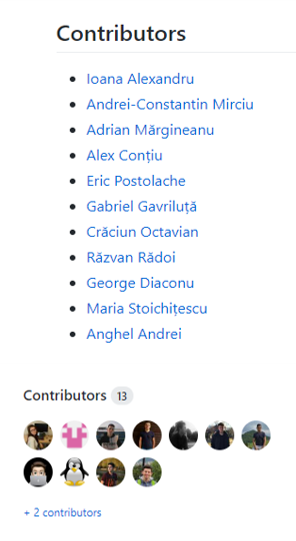
\includegraphics[width=0.42\columnwidth]{figures/contributors.png}
            \captionsetup{labelsep=space, textformat=empty}
            \caption{Application contributors according to GitHub}
            \label{2:fig:contributors}
    \end{wrapfigure}

    Although it started as a simple personal project, the desire of the founders of this idea pushed them to take everything to a higher level. Wanting to ensure that this application was published in the shortest time possible and realizing that development on their own is far from being effective, it was concluded that a team was necessary.
    
    Starting in July 2020, Ioana Alexandru, the initiator of this project, managed to structure a squad of about six people willing to contribute in their spare time, regardless of the year of study.
    
    Initially, all the participants gathered were trained through a \textit{workshop}\footnote{https://github.com/student-hub/flutter-workshop} about the purpose of this idea and familiarized with the technology used and the structure of the existing codebase. Subsequently, they were proposed diverse directions in which to get involved voluntarily, depending on the preferences and knowledge of each one. Among the aspects proposed, we can identify ideas that involve implementing new features or fixing known bugs \& issues, research on User Experience (\textit{\acrshort{ux}}) and User Interface (\textit{\acrshort{ui}}) design, the addition of relevant information into the database, and improving the code testing approach.
    
    Until the beginning of the next academic year in October 2020, this team kept expanding, all students being united by the same passion, more precisely the development of a handy and straightforward to use, comprehensive product, respecting the slogan \textit{from students, for students}. To maintain an organized structure regarding their progress, they decided to establish a weekly meeting to discuss the contribution of each team member during the previous week and also mention which objectives to focus on next.
    
    The author of the current thesis is part of the team of developers built around this idea. Thereupon, we will use the pronoun \textit{our} to refer to the work environment of this project.
    
    Due to the pandemic context, our communication was based exclusively online, via platforms like \textit{WhatsApp}\footnote{https://www.whatsapp.com/}, \textit{Google Meet}\footnote{https://meet.google.com/}, \textit{Slack}\footnote{https://slack.com/}, and \textit{Microsoft Teams}\footnote{https://teams.microsoft.com/}. However, this fact did not represent an impediment to achieving a realistic, friendly, and motivating work environment.
    
    About a year after being created, the team coordinating this project consists of more than ten active developers, and it is still growing (fig. \ref{2:fig:contributors}).
    
\subsection{Innovation Labs} \label{1:innovation_labs}

    Encouraged by the positive feedback received, we decided to advertise our idea to the general public from Romania by entering the \textbf{Innovation Labs}\footnote{https://www.innovationlabs.ro/} start-up accelerator program.
    
    Following the discussions with mentors from different areas of the industry, including education, marketing, and engineering, we concluded that it would be appropriate to create an association around this idea, namely \textbf{StudentHub}. We are planning to register our identity by the end of July 2021 officially.
    
    Correspondingly, this program facilitated a solid development of the application by constantly providing feedback on our progress and plans. Our team is currently developing a generic \textit{prototype}\footnote{https://github.com/student-hub/demo}, which can be used as a skeleton or backbone project to customize one single application concept for different universities in our country, depending on their specific requirements. Therefore, we permanently consider different architectural solutions to write code in a modular fashion, thus allowing easy decoupling of functionalities or data structures, if needed. Additional details about our architecture are described in chapter \ref{chapter5}. 
        
\section{Proposed functionalities} \label{1:functionalities}

    Following the circumstances previously illustrated in section \ref{1:environment}, the current thesis focuses on understanding the challenges students face daily and their opinion on the relevance of providing feedback for both teachers and their fellows.
    
    We collected and analyzed answers from students through a questionnaire distributed in an online fashion via social networks. We further present its outcome in chapter \ref{chapter3}, based on which we come up with ideas for improvement and structure the needs of students into technical specifications.
    
    Moreover, we designed, developed, validated, and integrated multiple modules with an already existing application, namely ACS UPB Mobile\footnote{https://github.com/student-hub/acs-upb-mobile}:
    
    \begin{itemize}
            \setlength{\topsep}{0.5pt}
            \setlength{\itemsep}{0.5pt}
            \setlength{\parsep}{0.5pt}
            \item people page located in the bottom navigation view, which contains handy and highly sought after contact details of teachers, displayed through a modal bottom sheet 
            \item search bar option that allows finding a specific person directly
            \item the connection between a lecture and its associated professor when a new event is added to the timetable
            \item card containing the class name and its corresponding lecturer on the class information page
            \item feedback form that can be accessed exclusively under certain conditions, mainly concerning specific periods
            \item a checklist page, which separates the classes depending on whether a student completed or not its matching feedback questionnaire; along with this feature, we created a notification card displaying the total number of reviews that are still pending to be concluded
            \item a statistics page with all the results gathered from students
\end{itemize}

    Hence, our application provides students transparency and relevant statistics and details about their classes through clear and concise pages. This approach broadens the awareness of students, as well as their overall level of information. Similarly, our features relieve older generations from presenting detailed descriptions about classes at the beginning or over a semester. At the moment, this type of action is time-consuming and takes place in a somewhat disorganized manner.

    Our work is sustained by an ecosystem that uses production-ready mechanisms, both in design and architecture, further detailed in chapters \ref{chapter4} and \ref{chapter5}. These help us increase our efficiency, consistency, and global quality by offering already predefined graphic elements, core functionalities, and lower operating costs, which are also presented in the previously mentioned chapters.

\section{Outline} \label{1:outline}

    \textbf{Chapter \ref{chapter2}} outlines the current context of the relevance of feedback in the educational system, looking both from our faculty of choice and other universities in conjunction with the pre-university environment in Romania. In the same manner, this chapter describes some concrete examples which support the usefulness of this idea.
    
    \textbf{Chapter \ref{chapter3}} highlights the methods used to obtain the opinion of students on the topic approached, focusing primarily on the analysis of a study conducted in this regard.
    
    \textbf{Chapter \ref{chapter4}} presents the stages preceding the beginning of the effective development of proposed functionalities, including prototype defining and the thinking behind the choice of questions from the feedback form.
    
    \textbf{Chapter \ref{chapter5}} exposes the architecture used, along with the database model. More than that, we indicate our automatic testing methods used to verify that our application is running smoothly. 
    
    \textbf{Chapter \ref{chapter6}} infers all conclusions reached following the analysis of the current thesis, along with ideas worthy of further consideration.